\documentclass[12pt, onecolumn]{memoir}
\usepackage{hyperref}
\usepackage{memhfixc}
\usepackage{graphicx}
\usepackage[utf8]{inputenc}
\usepackage[english]{babel}
\usepackage{amsmath,amssymb}
\usepackage[final]{microtype}
\usepackage{color,calc,soul}
\usepackage{listings}
\usepackage{tikz}
\usetikzlibrary{arrows}
\usetikzlibrary{trees}
\usepackage{tikzorbital}
\usepackage{supertabular}
\usepackage{gensymb}
\usepackage{apacite}

\newcommand*{\doi}{}
\makeatletter
\newcommand{\doi@}[1]{\href{https://doi.org/#1}{#1}}
\DeclareRobustCommand{\doi}{\hyper@normalise\doi@}
\makeatother

\tikzstyle{lien}=[->,>=stealth,rounded corners=5pt,thick]
\tikzset{individu/.style={draw,thick,fill=#1!25},
individu/.default={green}}

\definecolor{nicered}{rgb}{.647,.129,.149}
\makeatletter
\newlength\dlf@normtxtw
\setlength\dlf@normtxtw{\textwidth}
\def\myhelvetfont{\def\sfdefault{mdput}}
\newsavebox{\feline@chapter}
\newcommand\feline@chapter@marker[1][4cm]{%
  \sbox\feline@chapter{%
    \resizebox{!}{#1}{\fboxsep=1pt%
      \colorbox{nicered}{\color{white}\bfseries\sffamily\thechapter}%
    }}%
  \rotatebox{90}{%
    \resizebox{%
      \heightof{\usebox{\feline@chapter}}+\depthof{\usebox{\feline@chapter}}}%
    {!}{\scshape\so\@chapapp}}\quad%
  \raisebox{\depthof{\usebox{\feline@chapter}}}{\usebox{\feline@chapter}}%
}
\newcommand\feline@chm[1][4cm]{%
  \sbox\feline@chapter{\feline@chapter@marker[#1]}%
  \makebox[0pt][l]{% aka \rlap
    \makebox[1cm][r]{\usebox\feline@chapter}%
  }}
\makechapterstyle{daleif1}{
  \renewcommand\chapnamefont{\normalfont\Large\scshape\raggedleft\so}
  \renewcommand\chaptitlefont{\normalfont\huge\bfseries\scshape\color{nicered}}
  \renewcommand\chapternamenum{}
  \renewcommand\printchaptername{}
  \renewcommand\printchapternum{\null\hfill\feline@chm[2.5cm]\par}
  \renewcommand\afterchapternum{\par\vskip\midchapskip}
  \renewcommand\printchaptertitle[1]{\chaptitlefont\raggedleft ##1\par}
}

\newenvironment{liste}{\begin{itemize}
\renewcommand{\labelitemi}{}}{\end{itemize}}
\newcommand{\ra}{\rightarrow}
\newcommand{\hlin}{ & & \\ \hline  }
\newcommand{\linksec}[1]{\hyperref[#1]{\ref{#1}}   }

\renewcommand{\sectionmark}[1]{\markboth{\thesection.\ #1}{}}
\renewcommand{\subsectionmark}[1]{\markright{\thesubsection\ #1}}

\newcommand{\TBK}{\textcolor{nicered}{TBKOSTER}}
\makeatother

\title{{\textbf{\huge\TBK}} \\ \textsc{\small Tight-Binding Magnetic Molecular Dynamics for everyone}}
\author{C. Barreteau, P. Thibaudeau \thanks{Supported by CEA}}
\date{Release 0.0.4\\ \today}

\begin{document}
\frontmatter
\maketitle
%\begin{abstract}
%\end{abstract}
\vfil
\pagebreak
\let\clearforchapter\par %Comment this at the end
\chapterstyle{daleif1}

\tableofcontents*

\vfil
\pagebreak

\chapter*{Preface}
This manual describes the {\TBK} computer code. 

\begin{center}
  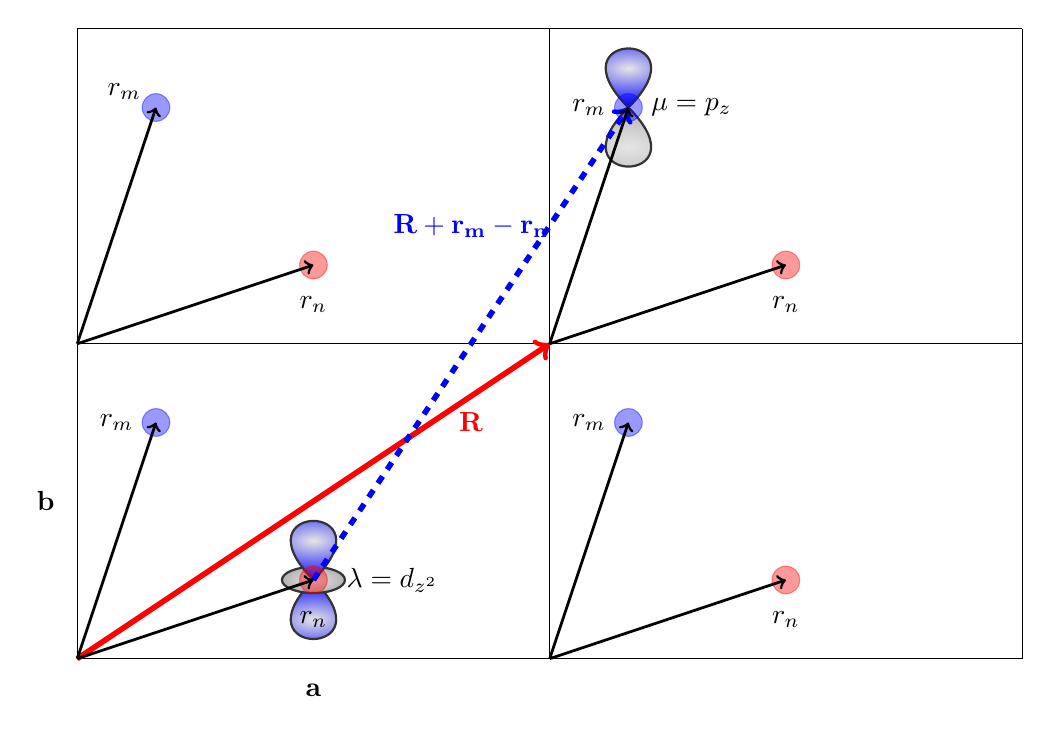
\begin{tikzpicture}
  \draw  (0,0)-- (12,0);
  \draw  (0,0)-- (0,8);
  \draw  (0,8)-- (12,8);
  \draw  (12,0)-- (12,8);
  \draw  (0,4)-- (12,4);
  \draw  (6,0)-- (6,8);

  \draw[color=blue,fill=blue,opacity=0.4]  (1,3) circle (5pt);
  \draw[color=red,fill=red,opacity=0.4]    (3,1) circle (5pt);

  \draw[color=blue,fill=blue,opacity=0.4]  (7,7) circle (5pt);
  \draw[color=red,fill=red,opacity=0.4]    (9,5) circle (5pt);

  \draw[color=blue,fill=blue,opacity=0.4]  (1,7) circle (5pt);
  \draw[color=red,fill=red,opacity=0.4]    (3,5) circle (5pt);

  \draw[color=blue,fill=blue,opacity=0.4]  (7,3) circle (5pt);
  \draw[color=red,fill=red,opacity=0.4]    (9,1) circle (5pt);

  \draw [->,line width=2pt,color=red] (0,0) -- (6,4);
  \draw [->,line width=2pt,color=blue, dashed] (3,1) -- (7,7);
  \draw [->,line width=1pt] (0,0) -- (1,3);
  \draw [->,line width=1pt] (0,0) -- (3,1);
  \draw [->,line width=1pt] (6,4) -- (7,7);
  \draw [->,line width=1pt] (6,4) -- (9,5);
  \draw [->,line width=1pt] (0,4) -- (1,7);
  \draw [->,line width=1pt] (0,4) -- (3,5);
  \draw [->,line width=1pt] (6,0) -- (7,3);
  \draw [->,line width=1pt] (6,0) -- (9,1);

  \draw (3,-0.4) node {$\mathbf{a}$};
  \draw (-0.4,2) node {$\mathbf{b}$};

  \draw (0.5,3) node {$r_m$};
  \draw (3,0.5) node {$r_n$};
  \draw (6.5,7) node {$r_m$};
  \draw (9,4.5) node {$r_n$};
  \draw (6.5,3) node {$r_m$};
  \draw (9,0.5) node {$r_n$};
  \draw (0.6,7.2) node {$r_m$};
  \draw (3,4.5) node {$r_n$};

  \draw[color=red] (5,3) node {$\mathbf{R}$};
  \draw[color=blue] (5,5.5) node {$\mathbf{R+r_m-r_n}$};

  \orbital[pos = {(3,1)}]{dz2}
  \draw (4,1) node {$\lambda=d_{z^2}$};

  \orbital[pos = {(7,7)}]{pz}
  \draw (7.8,7) node {$\mu=p_z$};

  \end{tikzpicture}
\end{center}

\mainmatter

\chapter{Background theory}

This section displays references for computing the magnetic electronic structure in the tight-binding (TB) approximation, with several atoms per unit-cell, periodic boundary conditions and orbital overlaps.

\begin{itemize}
  \item[$\bullet$]{\textbf{General formalism} with several atoms per unit-cell, non-collinear magnetism, overlap orbital integrals and periodic boundary conditions is described thoroughly in the file \href{https://fr.overleaf.com/read/hvmmbjspmtcg#e8c298}{\textcolor{blue}{Formalism.pdf}}.}
  \item[$\bullet$]{\textbf{NRL-TB}: The NRL Tight-Binding method provides an efficient method for calculating properties of materials. The advantage of this method over classical interatomic potential simulations is that it explicitly incorporates the real electronic structure and bonding of the material, obtained by an interpolation from a database of first-principles results. The Hamiltonian and formalism is described in the review paper \cite{barreteauEfficientMagneticTightbinding2016}.} 
  \item[$\bullet$]{\textbf{Magnetic Force Theorem (MFT)} and its application to the calculation of magneto-crystalline anisotropy can be found in reference \cite{liMagnetocrystallineAnisotropyEnergy2013}.
  }
  \item[$\bullet$]{\textbf{Spin Dynamics} in the tight-binding formalism is described in reference \cite{cardiasSpinDynamicsConstrained2021}.
  } 
\end{itemize}
\vfil

\chapter{Installation}

\section{Download the code}

The first step is to download the latest release of TBKOSTER from its github repository. To proceed, you have to check that git is installed~:
\begin{lstlisting}[language=bash,basicstyle=\small\ttfamily]
$ locate git
\end{lstlisting}
Then, clone the distant repository to your local computer~:
\begin{lstlisting}[language=bash,basicstyle=\small\ttfamily]
$ git clone https://github.com/spindynamics/TBKOSTER.git
\end{lstlisting}
In order to build this documentation, a LaTeX distribution is mandatory, including some external packages such as pdflatex, bibtex and htlatex.
%%%%%%%%%%%%%%%%%%%%%%%
\section{Linux}
Preferred method : on Ubuntu 22.04 and later, install gfortran and cmake to compile TBKOSTER. Be sure to get the mandatory related dependencies of these packages.
\begin{lstlisting}[language=sh,basicstyle=\small\ttfamily,frame=single,breaklines=true]
$ sudo apt install cmake gfortran clang doxygen graphviz libopenblas-dev libomp-dev texlive-latex-base texlive-latex-extra texlive-bibtex-extra tex4ht biber
\end{lstlisting}
Be sure to update to cmake release 3.13 or higher.
In order to build the code, to the root of TBKOSTER directory~:
\begin{lstlisting}[language=sh,basicstyle=\small\ttfamily,frame=single]
  $ cd TBKOSTER
  $ cmake -B build
  $ cmake --build build
\end{lstlisting}
To get access to the OpenMP parallel feature of the code, be sure to update your packages with the openmp support.

If you want to use Intel compiler, MKL and Intel Lapack libraries, you have to swicth this to cmake as, in sequential :
\begin{lstlisting}[language=sh,basicstyle=\small\ttfamily]
$ BLA_VENDOR=Intel10_64lp_seq FC=ifort cmake -B build
\end{lstlisting}
Be sure that the variable MKLROOT is set accordingly.

In order to get good numerical performance, you have to produce a Release version as :
\begin{lstlisting}[language=sh,basicstyle=\small\ttfamily]
$ cmake -DCMAKE_BUILD_TYPE=Release -B build
\end{lstlisting}
You can combine all these options.
If you prefer to prepare an installation with a given installed Lapack library and gfortran try :
\begin{lstlisting}[language=sh,basicstyle=\small\ttfamily]
$ BLA_VENDOR=OpenBLAS FC=gfortran cmake -B build
\end{lstlisting}
%%%%%%%%%%%%%%%%%%%%%%%
\section{MacOS}
Preferred method: on MacOS 10.11 and later, install cmake, lapack and gfortran with llvm support, with the \href{https://www.macports.org}{ports} subsystem:
\begin{lstlisting}[language=sh,basicstyle=\small\ttfamily,frame=single]
$ sudo port install cmake gcc libgcc gcc_select \
llvm-3.9 llvm_select lapack libomp
\end{lstlisting}
\href{https://brew.sh}{Brew} is also a working alternative.
In order to build the code, to the root of TBKOSTER directory~:
\begin{lstlisting}[language=sh,basicstyle=\small\ttfamily,frame=single]
$ cd TBKOSTER
$ cmake -B build
$ cmake --build build
\end{lstlisting}
For both Linux and MacOS platform, you can invoke cmake with Release or Debug option in order to deploy these releases. Simply try
\begin{lstlisting}[language=sh,basicstyle=\small\ttfamily]
$ cmake -DCMAKE_BUILD_TYPE=Release/Debug -B build
\end{lstlisting}
To get access to the OpenMP implementation, then update your ports with openmp package. You can easily change your settings with (assuming MacOS port is installed)
\begin{lstlisting}[language=sh,basicstyle=\small\ttfamily,frame=single]
$ port select --summary
$ port select --set llvm mp-llvm-3.9
$ port select --set gcc mp-gcc6
\end{lstlisting}
In order to get good numerical performance, you may use the OpenBLAS library and produce a Release version as :
\begin{lstlisting}[language=sh,basicstyle=\small\ttfamily,frame=single]
$ port install openblas
$ BLA_VENDOR=OpenBLAS \
cmake -DCMAKE_BUILD_TYPE=Release -B build
\end{lstlisting}
%%%%%%%%%%%%%%%%%%%%
\section{MS Windows}
For Windows earlier than 10 release 1709, you have to consider the following method:
download and follow the instructions to install MSYS2 software distro and building platform (http://www.msys2.org/). Open an MSYS console and first upgrade the whole system~:
\begin{lstlisting}[language=sh,basicstyle=\small\ttfamily]
$ pacman -Syu
\end{lstlisting}
get the compilation toolchain~:
\begin{lstlisting}[language=sh,basicstyle=\small\ttfamily]
$ pacman -S mingw-w64-x86_64-toolchain
\end{lstlisting}
get the gfortran compiler and lapack library~:
\begin{lstlisting}[language=sh,basicstyle=\small\ttfamily,frame=single]
$ pacman -S mingw-w64-x86_64-gcc-libgfortran
$ pacman -S mingw-w64-x86_64-openblas
\end{lstlisting}
get the cmake program to control the software compilation process using simple platform and compiler independent configuration files, and to generate native makefiles and workspaces that can be used in the compiler environment of your choice~:
\begin{lstlisting}[language=bash,basicstyle=\small\ttfamily]
$ pacman -S cmake
\end{lstlisting}

In order to build the code, open a MSYS MINGW 64-bit console. To the root of TBKOSTER directory~:
\begin{lstlisting}[language=sh,basicstyle=\small\ttfamily,frame=single]
$ cmake -G"MinGW Makefiles" \
-DCMAKE_SH="CMAKE_SH-NOTFOUND" -B build
$ cd build && mingw32-make
\end{lstlisting}
In order to run TBKOSTER.exe, be sure you have the TERM and TERMINFO environment variables up to date into your .bashrc file~:
\begin{lstlisting}[language=sh,basicstyle=\small\ttfamily]
$ export TERM=xterm
$ export TERMINFO=/c/Program Files/msys/mingw64/share/terminfo
\end{lstlisting}
No OpenMP implementation for MS Windows has been tested.

For Windows higher than 10 release 1709, you simply have to activate the optional Windows SubSystem for Linux, download the Ubuntu Package from the Microsoft Marketplace and follow the instructions of the Linux section of this manual.
\vfil

\section{Additional features}
Experimental features are coming from the dev branch of TBKOSTER.
First install the \href{https://stdlib.fortran-lang.org/}{fortran stdlib}:
\begin{lstlisting}[language=bash,basicstyle=\small\ttfamily,frame=single]
$ python3 -m venv .venv
$ source .venv/bin/activate
$ pip install fypp
$ git clone https://github.com/fortran-lang/stdlib
$ cd stdlib
$ cmake -DCMAKE_INSTALL_PREFIX=$HOME/.local -Bbuild .
$ cmake --build build --parallel 4
$ cmake --install build 
\end{lstlisting}
The fortran stdlib is installed in your \$HOME/.local folder.
Return to TBKOSTER, switch to the dev branch and compile 
\begin{lstlisting}[language=bash,basicstyle=\small\ttfamily,frame=single]
$ cd TBKOSTER
$ git checkout dev
$ rm -fr build
$ cmake -Bbuild .
$ cmake --build build --parallel 4
\end{lstlisting}
During the process, the fortran stdlib has to be found.

\vfil
\pagebreak

\chapter{Running the code}

\section{Directories}

\tikzstyle{lien}=[->,>=stealth,rounded corners=5pt,thick]
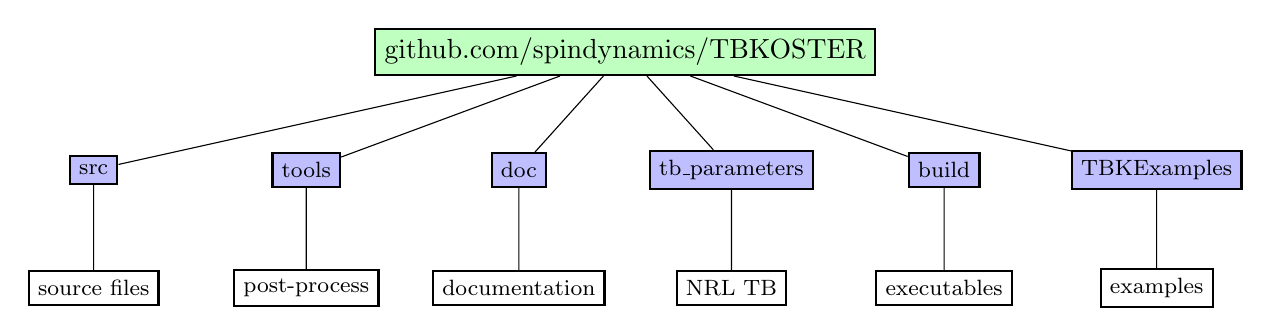
\begin{tikzpicture}
[level 1/.style={sibling distance=2.7cm},
level 2/.style={sibling distance=2.7cm}]
\node [individu] {github.com/spindynamics/TBKOSTER}
child { node [individu=blue]{\footnotesize{src}}
child { node [individu=white]{\footnotesize{source files}}}}
child { node [individu=blue]{\footnotesize{tools}}
child { node [individu=white]{\footnotesize{post-process}}}}
child { node [individu=blue]{\footnotesize{doc}}
child { node [individu=white]{\footnotesize{documentation}}}}
child { node [individu=blue]{\footnotesize{tb\_parameters}}
child { node [individu=white]{\footnotesize{NRL TB}}}}
child { node [individu=blue]{\footnotesize{build}}
child { node [individu=white]{\footnotesize{executables}}}}
child { node [individu=blue]{\footnotesize{TBKExamples}}
child { node [individu=white]{\footnotesize{examples}}}}
;
\end{tikzpicture}

\section{build directory}

The \textit{build} directory contains all the necessary binaries and documentation.

\section{running TBKOSTER}
\label{sec:Running}

{\TBK} needs an \verb+in_master.txt+ file to run. 
\verb+in_master.txt+ contains all the parameters of the calculation. 
This file is described in details in the section \ref{sec:Input_files}.

\vfil
\pagebreak

\chapter{Getting Started}
\label{sec:Getting_Started}

To get started, first we recommend to run the various examples that are provided within the TBKOSTER project.
\begin{lstlisting}[language=bash,basicstyle=\small\ttfamily,frame=single,breaklines=true]
$git clone https://github.com/spindynamics/TBKExamples 
\end{lstlisting}
In the directory TBKExamples, you have to update the location of the folder where to find the TBKOSTER binaries in the file 
\textit{environment\_variables}.
Update the {\textit{TBKOSTER\_ROOT}} variable.
This directory is organized as follow;

\vspace{0.5cm}

\noindent
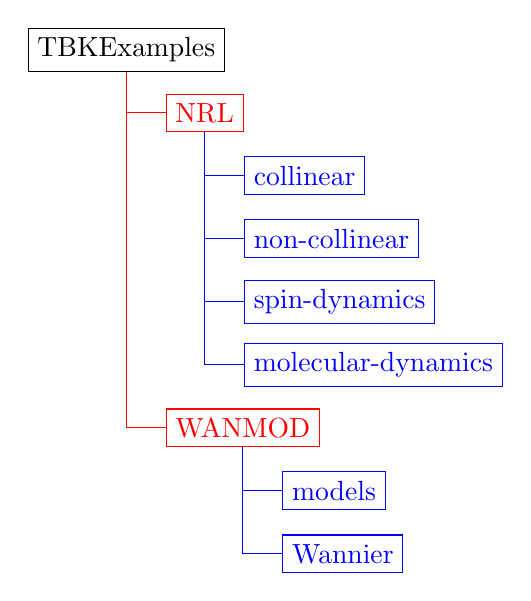
\begin{tikzpicture}
[
	level 1/.style = {red},
	level 2/.style = {blue},
	level 3/.style = {teal},
	every node/.append style = {draw, anchor = west},
	grow via three points={one child at (0.5,-0.8) and two children at (0.5,-0.8) and (0.5,-1.6)},
	edge from parent path={(\tikzparentnode\tikzparentanchor) |- (\tikzchildnode\tikzchildanchor)}]

\node {TBKExamples}
	child {node {NRL}
	child {node {collinear}}
	child {node {non-collinear}}
  child {node {spin-dynamics}}
	child {node {molecular-dynamics}}}
  child [missing] {}
  child [missing] {} 
  child [missing] {} 
  child [missing] {}  
	child {node {WANMOD}
	child {node {models}}
	child {node {Wannier}}};
\end{tikzpicture}

\vspace{0.5cm}

\noindent
Each \textcolor{nicered}{sub-directory} contains a \verb+README.md+ file and a list of directories labelled examplesxx, containing a script file called \verb+jobs.sh+.
This \verb+jobs.sh+ can be executed by the command \verb+./jobs.sh+
\vfil
\pagebreak

\chapter{I/O Command Reference}

\section{Input files}
\label{sec:Input_files}

\subsection{in\_master.txt}
The file \verb+in_master.txt+ is the main input file of \TBK.
\vfil

\begin{supertabular}{@{\hspace{0.025\textwidth}} p{0.15\textwidth} @{\hspace{0.025\textwidth}} 
p{0.3\textwidth} @{\hspace{0.025\textwidth}} p{0.65\textwidth} @{} }
& & \\
\hline
\hline
namelist &Variable     &Description\\
\hline 
\&calculation &  &\\
\hline
 & \verb+pre_processing+  (char)    & type of pre-processing calculation: 
                            \begin{liste} 
                                       \item 'txt2xyz'$\ra$ write geometry in xyz format, 
                            \end{liste} \\
& \verb+pre_processing_dir+  (char)    & directory for saving pre-processing calculation: 
                            \begin{liste} 
                                       \item 'txt2xyz'$\ra$ default value, 
                            \end{liste} \\

 & \verb+processing+  (char)    & type of processing calculation: 
                            \begin{liste} 
                                       \item 'scf'$\ra$ \textbf{self-consistent}, 
                                       \item 'md'$\ra$ molecular-dynamics. 
                                       \item 'sd'$\ra$ spin-dynamics. 
                            \end{liste} \\
 & \verb+post_processing+  (char)    & type of post-processing calculation (always preceded by a scf calculation): 
                            \begin{liste} 
                                       \item 'band'$\ra$ band structure calculation, 
                                       \item 'dos'$\ra$ density of states calculation. 
                                        \item 'forces'$\ra$ forces calculation. 
                                       \item 'mft'$\ra$ magnetic force theorem. 
                            \end{liste} \\
\hline
\&units &  &   \\
\hline

 & \verb+energy+  (char)  &  Energy unit:   
                          \begin{liste}    
                                   \item 'hau'$\ra$ \textbf{Hartree atomic units }, 
                                   \item 'rau'$\ra$ Rydberg atomic units, 
                                    \item 'ev'$\ra$ electronvolts. 
                           \end{liste} \\
 & \verb+length+  (char)  &  Length unit:   
                          \begin{liste}    
                                   \item 'hau'$\ra$ \textbf{Hartree atomic units}, 
                                   \item 'rau'$\ra$ Rydberg atomic units, 
                                   \item 'nm'$\ra$ nanometer. 
                                   \item 'ang'$\ra$ angstrom. 
                           \end{liste} \\
  & \verb+time+  (char)  &  time unit:   
                          \begin{liste}    
                                   \item 'hau'$\ra$ \textbf{Hartree atomic units}, 
                                   \item 'rau'$\ra$ Rydberg atomic units, 
                                   \item 'fs'$\ra$ femtoseconds. 
                           \end{liste} \\             
 & \verb+mass+  (char)  &  Mass unit:   
                          \begin{liste}    
                                   \item 'hau'$\ra$ \textbf{Hartree atomic units}, 
                                   \item 'rau'$\ra$ Rydberg atomic units, 
                                   \item 'g/mol'$\ra$ g/mol. 
                           \end{liste} \\

\hline
\&element &  &   \\
\hline                       
 & \verb+ne+  (int) &  Number of different elements in the system. 
  \\ 
 & \verb+symbol(i)+  (char) &  Symbol of the elements in the system  $i=1,\cdots,ne$ 
 \\
 & \verb+no(i)+  (int) &  number of orbitals of element $i=1,\cdots,ne$ (optional)
 \\
 & \verb+o(i,1:no(i))+ (int) &  list of orbitals $i=1,\cdots,ne$ 
 \\
 & \verb+q(i)+  (real) &   input charge of element \nolinebreak$i=1,\cdots,ne$ 
 \\
  & \verb+q_s(i)+  (real) &  $s$ input charge of element \nolinebreak$i=1,\cdots,ne$ 
 \\
  & \verb+q_p(i)+  (real) &  $p$ input charge of element \nolinebreak$i=1,\cdots,ne$
 \\
 & \verb+q_d(i)+  (real) &  $d$ input charge of element \nolinebreak$i=1,\cdots,ne$
 \\
  & \verb+u_lcn(i)+  (real) &  U (in eV) value of element \nolinebreak$i=1,\cdots,ne$ for local charge neutrality
 \\
   & \verb+u_lcn_d(i)+  (real) &  Ud (in eV) value of element \nolinebreak$i=1,\cdots,ne$ for local $d$ charge neutrality
 \\
 & \verb+i_stoner_d(i)+  (real) &  Stoner parameter of element \nolinebreak$i=1,\cdots,ne$ for of $d$ orbitals for magnetic systems.
 \\
  & \verb+xi_so_p(i)+  (real) &  spin-orbit coupling constant of element $i=1,\cdots,ne$ for $p$ orbitals
 \\
 & \verb+xi_so_d(i)+  (real) &   spin-orbit coupling constant of element $i=1,\cdots,ne$ for $d$ orbitals
 \\
 \hline
\&element\_tb &  &   \\
\hline      
 & \verb+tb_type+  (char) &  type of TB calculation
                        \begin{liste}    
                                   \item 'nrl'$\ra$ \textbf{NRL TB}, 
                                   \item 'mod'$\ra$ model TB (input=mod.dat), 
                                    \item 'wan'$\ra$ Wannier TB (input=hr.dat). 
                           \end{liste} \\
 & \verb+filename(i)+  (char) &  file with the NRL TB parameters of element $i=1,\cdots,ne$.
 \\        
 \hline
\&lattice &  &   \\
\hline                       
 & \verb+v_factor+  (real) &  Multiplication factor applied to the lattice vectors. 
  \\ 
 & \verb+v(1:3,3)+  (real) & 3 translation vectors $\mathbf{a}=v(1,:)$,$\mathbf{b}=v(2,:)$,$\mathbf{c}=v(3,:)$, 
 \\
 \hline
\&atom &  &   \\
\hline                       
 & \verb+ns+  (int) &  Type of magnetic system. 
   \begin{liste}    
                             \item '1'$\ra$ \textbf{non magnetic system}, 
                             \item '2'$\ra$ collinear spin, 
                             \item '4'$\ra$ non-collinear spin. 
 \end{liste} \\
 & \verb+na+  (int) &  Number of atoms in the system. 
 \\
  & \verb+k_spiral(3)+  (real) &  spiral vector for spin-spiral calculations (defaut k\_spiral=(0,0,0)). 
 \\
  & \verb+ntag+  (int) &  Number of tags to give names to differents atoms. 
 \\
  & \verb+stag(i)+  (int) &  Number of atoms of tag $i=1,\cdots,ntag$. 
 \\
   & \verb+tag(i)+  (char) &  tag of atom $i=1,\cdots,ntag$. 
 \\
 & \verb+pbc(3)+  (int) &  number of unit-cell in the three periodic directions to search for neighbours. if pbc($i$)=0 then there is no periodicity in direction $i$. 
 \\
 &\verb+r_coord+ (char) & type of coordinate for atom positions,
\begin{liste}  
                        \item '\textbf{direct}'$\ra$ in fractions of $a$, $b$ and $c$ coordinate, 
                        \item 'cartesian'$\ra$ $xyz$ coordinates, 
\end{liste} \\ 
 & \verb+x(i,3)+  (real) & coordinates of atom $i=1,\cdots,na$, 
 \\
 &\verb+m_coord+ (char) & type of coordinate for magnetism,
\begin{liste}  
                        \item '\textbf{spherical}'$\ra$ $m$, $\theta$ and $\phi$ coordinate, 
                        \item 'cartesian'$\ra$ $xyz$ oordinates, 
\end{liste} \\ 
 &\verb+m_listing+ (char) & type of magnetic assignation,
\begin{liste}  
                        \item '\textbf{by\_atom}'$\ra$ by atom, 
                        \item 'by\_tag'$\ra$ by tag, 
\end{liste} \\ 
 & \verb+m(i,3)+  (real) & magnetic coordinates of atom $i=1,\cdots,na$ or $i=1,\cdots,ntag$
 \\
  &\verb+lambda_pen_listing+ (char) & type of magnetic assignation,
\begin{liste}  
                        \item '\textbf{by\_atom}'$\ra$ by atom, 
                        \item 'by\_tag'$\ra$ by tag, 
\end{liste} \\ 
  & \verb+lambda_pen(i)+  (real) & magnetic penalization factor of atom $i=1,\cdots,na$ or $i=1,\cdots,ntag$
 \\
 \hline
\&mesh &  &   \\
\hline        
 & \verb+type+  (char) &  type of $k$ mesh
                        \begin{liste}    
                                   \item '\textbf{mp}'$\ra$ monkhorst pack mesh, 
                                   \item 'path'$\ra$ path in k-space, 
                                    \item 'list'$\ra$ list of $k$-vectors. 
                           \end{liste} \\
 & \verb+x_coord+  (char) &  type of $k$ mesh
                        \begin{liste}    
                        \item '\textbf{direct}'$\ra$ in fractions of $a$, $b$ and $c$ coordinate, 
                        \item 'cartesian'$\ra$ $xyz$ coordinates, 
                           \end{liste} \\
 & \verb+gx(3)+  (int) &   $gx=(n_a,n_b,n_c)$, $n_i$ integer, when type=mp.
 \\
 & \verb+dx(3)+  (int) &   $dx=(d_a,d_b,d_c)$ $d_i=0,1$ shift when type=mp.
 \\
  & \verb+nxs+  (int) &   number of symmetry point when type=path.
 \\
  & \verb+gxs+  (int) &   number of points between two consecutive symmetry-point when type=path.
 \\
 & \verb+xs(1:nxs,3)+  (int) &   coordinate of the symmetry points when type=path
 \\
 & \verb+xs_label(1:nxs)+  (int) &   label (G,X,M,K etc..) of the symmetry points when type=path
 \\
 & \verb+nx+  (int) &      number of $k$ points when type=list.
 \\
  & \verb+x(1:nx,3)+  (int) &   coordinate of the $k$ points when type=list
 \\                   
 \\
 \hline
\&hamiltonian\_tb &  &   \\
\hline     
& \verb+e_e_interaction+  (char) &  type of electronic interaction
                        \begin{liste}    
                                   \item '\textbf{stoner}'$\ra$ monkhorst pack mesh, 
                                   \item 'ujb'$\ra$ TB+U(J,B), 
                           \end{liste} \\
& \verb+m_penalization+  (char) &  type of magnetic penalization
                        \begin{liste}    
                                   \item '\textbf{none}'$\ra$ no penalization 
                                   \item 'r'$\ra$ penalization of the amplitude of the spin moment $m(i)$ for each atom.
                                   \item 'r,$\theta$'$\ra$ penalization of the amplitude of the spin moment $m(i)$  and on the $\theta(i)$ angle for each atom.
                                   \item 'r,$\theta$,$\phi$'$\ra$ penalization of the amplitude of the spin moment $m(i)$  and on the $\theta(i)$ and $\phi(i)$ angles for each atom.
                                    \item '$\theta$'$\ra$ penalization of the the $\theta(i)$ angle for each atom.
                                   \item '$\theta$,$\phi$'$\ra$ penalization of the $\theta(i)$ and $\phi(i)$ angles for each atom.
                                    \item '$\phi$'$\ra$ penalization of the $\phi(i)$ angles for each atom.
                           \end{liste} \\
 \hline
\&energy &  &   \\
\hline     
& \verb+smearing+  (char) &  type of smearing
                        \begin{liste}    
                                   \item '\textbf{mp}'$\ra$ Methfessel Paxton, 
                                   \item 'fd'$\ra$ Fermi Dirac, 
                                   \item 'mv'$\ra$ Marzari-Venderbilt, 
                                    \item 'g'$\ra$ Gaussian, 
                           \end{liste} \\
  & \verb+degauss+  (real) &   electronic broadeding
 \\  
  & \verb+fixed_fermi_level+  (logical) &   
   \begin{liste}    
                                   \item '\textbf{false}'$\ra$ Fermi level determined by number of electrons in the system, 
                                   \item 'true'$\ra$ Fermi level fixed to a given value \verb+en_f_ffl+, 
                           \end{liste} \\
                           
  & \verb+en_f_ffl+ (entier) &  value of the fixed "Fermi level" if fixed\_fermi\_level=true \\     
  & \verb+fixed_spin_moment+  (logical) &   
   \begin{liste}    
                                   \item '\textbf{false}'$\ra$ , 
                                   \item 'true'$\ra$ Fermi spin moment calculation, the total magnetization being equal to \verb+m_fsm+, \end{liste} \\
                           
  & \verb+m_fsm+ (entier) &  value of the fixed spin moment when fixed\_spin\_moment=true \\ 
 \hline
\&mixing &  &   \\
\hline     
& \verb+type+  (char) &  type of smearing
                        \begin{liste}    
                                   \item '\textbf{broyden}'$\ra$ Broyden mixing 
                                   \item 'linear'$\ra$ linear mixing, 
                           \end{liste} \\
  & \verb+alpha+  (real) &   mixing coefficient $0<\alpha<1$
 \\  
  & \verb+n_init+  (int) &  first step of Broyden mixing  (default 1)
 \\
   & \verb+n_hist+  (int) &  number of history steps of Broyden mixing (default 50)
 \\    
  \hline
\&scf &  &   \\
\hline     
& \verb+verbose+  (logical) &  type of smearing
                        \begin{liste}    
                                   \item '\textbf{false}'$\ra$ minimum writing in out\_log.txt file 
                                   \item 'true'$\ra$ verbose writing in out\_log.txt file, 
                           \end{liste} \\
  & \verb+delta_en+  (real) &   energy crtiterium for scf calculation
 \\ 
   & \verb+delta_q+  (real) &   charge crtiterium for scf calculation
 \\ 
  & \verb+ni_min+  (int) &  miniumum number of iteration (default 2)
 \\
   & \verb+ni_max+  (int) &  maximum number of iteration (default 50)
 \\                          
\hline
\hline
\end{supertabular}

\subsection{post-processing}

\subsubsection{ a) band}

\begin{center}\verb+band/in_band.txt  +\end{center}
\vspace{-0.5cm}

\begin{supertabular}{@{\hspace{0.025\textwidth}} p{0.15\textwidth} @{\hspace{0.025\textwidth}} 
p{0.3\textwidth} @{\hspace{0.025\textwidth}} p{0.65\textwidth} @{} }
& & \\
\hline
\hline
namelist &Variable     &Description \\
\hline 
\&band &  &   \\
\hline        
 & \verb+proj+  (char) &  type of projection
                        \begin{liste}    
                                   \item '\textbf{none}'$\ra$ no projection, 
                                   \item 'site'$\ra$ atomic site projection, 
                                    \item 'spin'$\ra$ spin projection (only if $ns=4$) to plot  spin-textures. 
                                     \item 'orbit'$\ra$ orbit projection (only if $ns=4$) to plot  orbit-textures. 
                                      \item 'spin,orbit'$\ra$ spin and orbit projection (only if $ns=4$) to plot  spin and orbit-textures.
                           \end{liste} \\
 & \verb+i_min+  (int) &  lowest band index to include in the calculation (default $i_min=1$) \\
  & \verb+i_max+  (int) &  largest band index to include in the calculation (default $i_max=nmax$)\\
 & \verb+na_band+  (int) &  number of atomic sites on which projection should be done (default na\_band=0).
 \\
 & \verb+ia_band(1:na_band)+  &  index of the atomic sites.
 \\                   
\hline
\hline
\end{supertabular}

\vspace{1cm}
\begin{center}\verb+band/in_mesh.txt  +\end{center}
\vspace{-0.5cm}

\noindent
Note that for band-structure calculation, although the type of mesh is by default \verb+type+=\textbf{mp}, band structure should be performed either with verb+type+=\textbf{path} or verb+type+=\textbf{list}. 


$\bullet$ \textbf{path} is used for "traditional" band-structure plotting

$\bullet$ \textbf{list} is used for 2D plot of spin, orbit or velocity textures.

\begin{supertabular}{@{\hspace{0.025\textwidth}} p{0.15\textwidth} @{\hspace{0.025\textwidth}} 
p{0.3\textwidth} @{\hspace{0.025\textwidth}} p{0.65\textwidth} @{} }
& & \\
\hline
\hline
namelist &Variable     &Description \\
\hline 
\hline        
 & \verb+type+  (char) &  type of $k$ mesh
                        \begin{liste}    
                                   \item '\textbf{mp}'$\ra$ monkhorst pack mesh, 
                                    \item 'path'$\ra$ path in k-space, 
                                    \item 'list'$\ra$ list of $k$-vector,
                           \end{liste} \\
 & \verb+x_coord+  (char) &  type of $k$ mesh
                        \begin{liste}    
                        \item '\textbf{direct}'$\ra$ in fractions of $a$, $b$ and $c$ coordinate, 
                        \item 'cartesian'$\ra$ $xyz$ coordinates, 
                           \end{liste} \\
 & \verb+gx(3)+  (int) &   $gx=(n_a,n_b,n_c)$, $n_i$ integer, when type=mp.
 \\
 & \verb+dx(3)+  (int) &   $dx=(d_a,d_b,d_c)$ $d_i=0,1$ shift when type=mp.
 \\
  & \verb+nxs+  (int) &   number of symmetry point when type=path.
 \\
  & \verb+gxs+  (int) &   number of points between two consecutive symmetry-point when type=path.
 \\
 & \verb+xs(1:nxs,3)+  (int) &   coordinate of the symmetry points when type=path
 \\
 & \verb+xs_label(1:nxs)+  (int) &   label (G,X,M,K etc..) of the symmetry points when type=path
 \\
 & \verb+nx+  (int) &      number of $k$ points when type=list.
 \\
  & \verb+x(1:nx,3)+  (int) &   coordinate of the $k$ points when type=list \\
\hline
\hline
\end{supertabular}

\subsubsection{ b) PDOS}

\vspace{0.5cm}
\begin{center}\verb+dos/in_dos.txt  +\end{center}
\vspace{-0.5cm}

\begin{supertabular}{@{\hspace{0.025\textwidth}} p{0.15\textwidth} @{\hspace{0.025\textwidth}} 
p{0.3\textwidth} @{\hspace{0.025\textwidth}} p{0.65\textwidth} @{} }
& & \\
\hline
\hline
namelist &Variable     &Description \\
\hline 
\&dos &  &   \\
\hline        
& \verb+nen+  (int) &  number of energy points \\
& \verb+na_dos+  (int) &  number of atomic sites on which the pdos will be projected\\
& \verb+ia(1:na_dos)+  (int) &  index of the sites.\\
& \verb+en_min+  (real) &  lower bound of energy window.\\
& \verb+en_max+  (real) &  upper bound of energy window.\\
 \\                   
\hline
\hline
\end{supertabular}

\vspace{0.5cm}
\begin{center}\verb+dos/in_energy.txt  +\end{center}
\vspace{-0.5cm}

\begin{supertabular}{@{\hspace{0.025\textwidth}} p{0.15\textwidth} @{\hspace{0.025\textwidth}} 
p{0.3\textwidth} @{\hspace{0.025\textwidth}} p{0.65\textwidth} @{} }
& & \\
\hline
\hline
namelist &Variable     &Description \\
\hline 
\&energy &  &   \\
\hline        
& \verb+smearing+  (char) &  smearing type
    \begin{liste}    
                                   \item '\textbf{mp}'$\ra$ Mathfessel Paxton, 
                                   \item 'mv'$\ra$ Marzari Vanderbilt, 
                                    \item 'fd'$\ra$ derivative of Fermi-Dirac. 
                                     \item 'g'$\ra$ Gaussian. 
\end{liste} \\
& \verb+degauss+  (real) &   broadening\\
 \\                   
\hline
\hline
\end{supertabular}

\vspace{0.5cm}

\begin{center}\verb+dos/in_mesh.txt +\end{center}

\vspace{-0.5cm}

\noindent
In \verb+dos/in_mesh.txt + all the options of \verb+&mesh+ are available however for PDOS one usually only use a MP k-point grid. Hence we have only listed below the most common parameters.


\begin{supertabular}{@{\hspace{0.025\textwidth}} p{0.15\textwidth} @{\hspace{0.025\textwidth}} 
p{0.3\textwidth} @{\hspace{0.025\textwidth}} p{0.65\textwidth} @{} }
& & \\
\hline
\hline
namelist &Variable     &Description \\
\hline 
\hline        
 & \verb+type+  (char) &  type of $k$ mesh
                        \begin{liste}    
                                   \item '\textbf{mp}'$\ra$ monkhorst pack mesh, 
                                   \item 'path'$\ra$ path in k-space, 
                                    \item 'list'$\ra$ list of $k$-vectors. 
                           \end{liste} \\
 & \verb+gx(3)+  (int) &   $gx=(n_a,n_b,n_c)$, $n_i$ integer, when type=mp.
 \\
 & \verb+dx(3)+  (int) &   $dx=(d_a,d_b,d_c)$ $d_i=0,1$ shift when type=mp.
 \\                   
\hline
\hline
\end{supertabular}

\subsubsection{ c) MFT (magnetic force theorem)}

The magnetic force theorem is used in two contexts: to evaluate the magnetocrystalline anisotropy or to compare the total energy of different magnetic configurations.

\begin{center}\verb+mft/in_mft.txt  +\end{center}
\vspace{-0.5cm}

\begin{supertabular}{@{\hspace{0.025\textwidth}} p{0.15\textwidth} @{\hspace{0.025\textwidth}} 
p{0.3\textwidth} @{\hspace{0.025\textwidth}} p{0.65\textwidth} @{} }
& & \\
\hline
\hline
namelist &Variable     &Description \\
\hline 
\&mft &  &   \\
\hline     
 & \verb+calc+  (char) &  type of calculation
                        \begin{liste}    
                                   \item '\textbf{mae}'$\ra$ magnetic anisotropy calculation, 
                                   \item 'mconfig'$\ra$ calculation of various magnetic non-collinear configurations, 
                           \end{liste} \\
 & \verb+type+  (char) &  type of mesh in $(\theta, \phi)$
                        \begin{liste}    
                                   \item 'mesh'$\ra$ regular mesh over the full spherical coordinates, 
                                   \item 'list'$\ra$ list of several $(\theta, \phi)$ angles, 
                                    \item 'path'$\ra$ path between various $(\theta, \phi)$ angles, 
                           \end{liste} \\                           
& \verb+na_mft+  (int) &  number of site on which the energy is projected (default na\_mft=0)\\
& \verb+ia(1:na_mfr)+  (int) &  index of the sites, if na\_mft=0 no need to specify all the indices.\\
& \verb+nxa+  (int) &  
$\bullet$ \textbf{calc=mae\&type=mesh}: (\verb+nxa+,\verb+nxa+) mesh over the spherical coordinates, \newline 
$\bullet$ \textbf{calc=mae\&type=path}: \verb+nxa+ is the number points between two angles, 
\newline 
$\bullet$ \textbf{calc=mae\&ype=list}: \verb+nxa+ is the number of angles in the list, 
\newline 
$\bullet$ \textbf{calc=mfonfig}: \verb+nxa+ is the number of magnetic configurations. \\
& \verb+mconfig(na,nxa,3)+  (real) &  define explicitly the \verb+nxa+ magnetic configurations over the \verb+na+ atoms of system\\
& \verb+nangle+  (int) &  in case type=path; nangle is the number of angles (\>2) to generate the path.\\
& \verb+angle_xs(nxa,3)+ (real) &  list of angles in spherical coordinates\\
 \\                   
\hline
\hline
\end{supertabular}

\newpage
%\vspace{0.5cm}
\begin{center}\verb+mft/in_energy.txt  +\end{center}
\vspace{-0.5cm}

\begin{supertabular}{@{\hspace{0.025\textwidth}} p{0.15\textwidth} @{\hspace{0.025\textwidth}} 
p{0.3\textwidth} @{\hspace{0.025\textwidth}} p{0.65\textwidth} @{} }
& & \\
\hline
\hline
namelist &Variable     &Description \\
\hline 
\&energy &  &   \\
\hline        
& \verb+smearing+  (char) &  smearing type
    \begin{liste}    
                                   \item '\textbf{mp}'$\ra$ Mathfessel Paxton, 
                                   \item 'mv'$\ra$ Marzari Vanderbilt, 
                                    \item 'fd'$\ra$ derivative of Fermi-Dirac. 
                                     \item 'g'$\ra$ Gaussian. 
\end{liste} \\
& \verb+degauss+  (real) &   broadening\\
 \\                   
\hline
\hline
\end{supertabular}

%\vspace{0.5cm}

\begin{center}\verb+mft/in_mesh.txt +\end{center}

\vspace{-0.5cm}

\noindent
In \verb+mesh/in_mesh.txt + all the options of \verb+&mesh+ are available however for MFT one only use a MP k-point grid. Hence we have only listed below the most common parameters.

\begin{supertabular}{@{\hspace{0.025\textwidth}} p{0.15\textwidth} @{\hspace{0.025\textwidth}} 
p{0.3\textwidth} @{\hspace{0.025\textwidth}} p{0.65\textwidth} @{} }
& & \\
\hline
\hline
namelist &Variable     &Description \\
\hline 
\hline        
 & \verb+type+  (char) &  type of $k$ mesh
                        \begin{liste}    
                                   \item '\textbf{mp}'$\ra$ monkhorst pack mesh, 
                                   \item 'path'$\ra$ path in k-space, 
                                    \item 'list'$\ra$ list of $k$-vectors. 
                           \end{liste} \\
 & \verb+gx(3)+  (int) &   $gx=(n_a,n_b,n_c)$, $n_i$ integer, when type=mp.
 \\
 & \verb+dx(3)+  (int) &   $dx=(d_a,d_b,d_c)$ $d_i=0,1$ shift when type=mp.
 \\                   
\hline
\hline
\end{supertabular}

\section{Output files}

\noindent
All the output files ( \verb+out_xxxx.txt+) of \TBK   
are in namelist format (except \verb+out_log.txt+), hence they can be re-used as input files for further calculations.


\subsection{out\_log.txt} 

 \noindent
\verb+out_log.txt+ is the main output file of \textcolor{nicered}{TBKOSTER}. The first lines of 
\verb+out_log.txt+ contains a summary of all the parameters (including the defaults) used for the calculation. Then, if \verb+verbosity=.true.+  \TBK print out in \verb+out_log.txt+ the charge and various quantities at each scf iteration. 

\subsection{out\_charge.txt}

 \noindent
\verb+out_charge.txt+ contains: \\

$\bullet$ the mulliken charge \verb+q_mul(1:na,1:3,0:ns-1)+

$\bullet$ and net charge \verb+rho_net(1:na,1:1:no,1:no,1:ns )+

 \noindent
 Importantly \verb+out_charge.txt+ can be copied in \verb+in_charge.txt+ whenever one needs a restart, for instance when a calculation is not fully converged.
 
\subsection{post-process output}

\subsubsection{a) txt2xyz}

\noindent
This option is used when one want to visualize the evolution of the  magnetic configuration during the scf cycle. This is particularly useful in the case of non-collinear magnetism. This option necessitate the setting of \verb+verbose=.true.+ in \verb+&scf+. \verb+out_atom_tb_xx.txt+ files are saved during the scf iterations. The \verb+txt2xyz+ option transforms the \verb+.txt+ file into \verb+.xyz+ that contain position and magnetization of atoms in the unit-cell. These files can be visualized via \verb+avogadro+ software to generate a movie showing the convergence process.

\subsubsection{b) dos}

\noindent
The main output file is \verb+dos/out_dos.txt+ file. It contains in namelist format:

$\bullet$ \verb+dos_tot(1:nE,1:ns)+: Total density of states

$\bullet$  \verb+dos_'orb'(1:na_dos,1:nE,1:ns)+: Projected density of states on different sites, different orbitals (orb=s,px, py etc..) and different spin index.

\subsubsection{c) band}

\noindent
The main output file is \verb+band/out_band.txt+ file. It contains in namelist format:

$\bullet$ \verb+en_k(1:nh,1:nk,1:ns)+: Eigenvalues \verb+nh+: size of Hamiltonian, \verb+nk+: number of $k$ points.

\textbf{If proj=site}

$\bullet$  \verb+w_band_site(1:nh,1:nk,1:na_band,1:norb,1:ns)+: weight of wavefunction on different sites, different orbitals and different spin index.

\textbf{If proj=spin}

$\bullet$  \verb+w_band_spin(1:nh,1:nk,0:na_band,1:4)+: average value of the Pauli matrices $\sigma_x, \sigma_y, \sigma_z$ (and its norm) for band index ih, $k$ point ik, site ia\_band.

\textbf{If proj=orbit}

$\bullet$  \verb+w_band_orb(1:nh,1:nk,0:na_band,1:4)+: average value of the orbital matrices $Lx, L_y, L_z$ (and its norm) for band index ih, $k$ point ik, site ia\_band.

\subsubsection{d) mft}

\noindent
The main output file is \verb+mft/out_mft_xxx.txt+ file. It contains for each magnetic configuration \verb+xxx+ in namelist format:

$\bullet$ \verb+mconfig(1:na,1:2)+: Magnetic configuration $(\theta, \phi)$ for each atom of the unit-cell

$\bullet$  \verb+mft_'orb'(1:na_mft)+: band energy projected on the selected sites for each orbitals (orb=s,px,py etc..).

$\bullet$  \verb+mft_sum+: Sum of the band energies projected on the selected sites of the unit-cell

$\bullet$  \verb+mft_tot+: Total band energy, it should be equal to \verb+mft_sum+ if \verb+nsite=na+


\subsection{tools output}

\noindent
The various tools read the output files of \TBK  in namelist format and reorganize them in a format directly readable by plotting software (\verb+xmgrace+, \verb+gnuplot+ etc..)

\subsubsection{a) pdos.x}

\noindent
\verb+pdos.x+ generates the following files:


$\bullet$ \verb+dos_tot.dat+: Total density of states

$\bullet$
\verb+pdos-s.dat+,  \verb+pdos-p.dat+, \verb+pdos-d.dat+ and \verb+pdos-spd.dat+: PDOS

\subsubsection{b) bands.x}

\noindent
\verb+bands.x+ generates different types of files depending on the options for the projection (proj) and for the type of mesh. 

\begin{center}
{\color{blue}\textbf{mesh=path}  }
\end{center}

\textbf{If proj=none}

$\bullet$
\verb+band.dat+: band structure along the $k$ path

\textbf{If proj=site}

$\bullet$
\verb+band.dat+: band structure along the $k$ path

$\bullet$
\verb+band_weight_site_orb.dat+: band structure along the $k$ PATH and associated weight on the defined sites.

\textbf{If proj=spin and/or proj=orb}

$\bullet$
\verb+band_weight_spinorb.dat+: band structure along the $k$ PATH and associated amplitude of the spin and/or orbit.


\begin{center}
{\color{blue}\textbf{mesh=list}  }
\end{center}

\noindent
Note that the "list" $k$-points are usually generated in cartesian coordinates via the \verb+build_kpoints.f90+ program. "list" mesh option is used to generate 2D maps

\textbf{If proj=spin and/or proj=orb}

\noindent
\verb+bands.x+ generates two files:

$\bullet$ \verb+fermi.dat+: 2D maps for Fermi surface

$\bullet$ \verb+fermi.dat+: 2D maps for "spin" or "orbit" vector field.

\subsubsection{c) mft.x}

\noindent
There are two type of MFT calculations: \verb+calc+= mae or \verb+calc+=mconfig.

\begin{center}
{\color{blue}\textbf{calc=mae}  }
\end{center}

\noindent
\verb+mft.x+ reads the \verb+out_mft_xxx.txt+ files and creates several files:

\textbf{If type=path}

$\bullet$
\verb+mae_angle.dat+: MAE along the $(\theta, \phi)$ path where the first angle of the path is taken as the reference zero energy.

$\bullet$
\verb+mae_atom.dat+: MAE energy decomposed on the different sites, and evaluated as the difference between the first and last magnetic orientation. 

$\bullet$
\verb+mae.xyz+: Same as \verb+mae_atom.dat+ but in $(x,y,z)$ coordinates.

\textbf{If type=mesh}

$\bullet$
\verb+mae_angle.dat+: MAE along the $(\theta, \phi)$ mesh where the first angle of the path is taken as the reference zero energy.

\begin{center}
{\color{blue}\textbf{calc=mconfig}}
\end{center}

\noindent
\verb+mft.x+ reads the \verb+out_mft_xxx.txt+ files and creates one summary file:

$\bullet$ \verb+mft_config.dat+ which contains the list of MFT band energies for the various configurations.
\vfil
\pagebreak
\bibliographystyle{apacite}
\bibliography{TBsd}
\appendix
\backmatter
\end{document}
